\documentclass[aspectratio=169]{beamer}
\usetheme[block=fill]{metropolis}
\usepackage{tikz}
\usetikzlibrary{shapes.geometric, arrows.meta, positioning, calc}

\title{Building a Reproducible Scholarly Search Toolkit}
\subtitle{Episode 9: Exponential Backoff \& Rate Limit Retries}
\author{Scholar Search Kit}
\date{}

\begin{document}

\begin{frame}[plain]
  \titlepage
\end{frame}

\begin{frame}{Episode Goal}
  \begin{alertblock}{The Goal}
    Implement smart decorators to automatically catch \texttt{SearchException}s and retry failed operations.
  \end{alertblock}
  \vspace{0.5cm}
  If an API drops our connection, we should silently wait and try again. If it tells us to slow down, we should obey exactly.
\end{frame}

\begin{frame}{The Decorator Pattern}
  \begin{center}
  \resizebox{0.7\linewidth}{!}{
  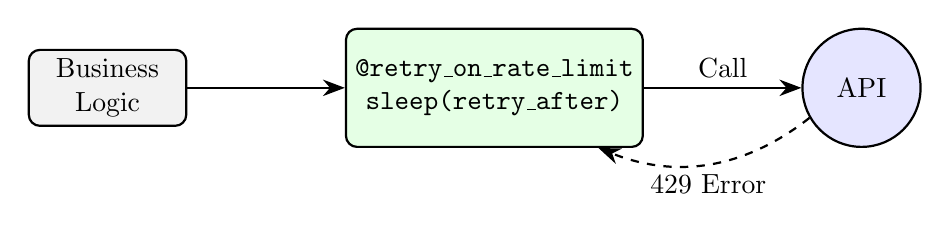
\begin{tikzpicture}[
      node distance=1.5cm and 2cm,
      caller/.style={rectangle, draw, thick, rounded corners, minimum width=2cm, align=center, fill=black!5},
      decorator/.style={rectangle, draw, thick, rounded corners, minimum width=3cm, minimum height=1.5cm, align=center, fill=green!10},
      api/.style={circle, draw, thick, minimum size=1.5cm, align=center, fill=blue!10},
      arrow/.style={-{Stealth[scale=1.2]}, thick}
    ]
    
    \node[caller] (c) {Business\\Logic};
    \node[decorator, right=of c] (d) {\texttt{@retry\_on\_rate\_limit}\\\texttt{sleep(retry\_after)}};
    \node[api, right=of d] (a) {API};
    
    \draw[arrow] (c) -- (d);
    \draw[arrow] (d) -- node[above] {Call} (a);
    \draw[arrow, dashed] (a) to[bend left] node[below] {429 Error} (d);
  \end{tikzpicture}
  }
  \end{center}
\end{frame}

\begin{frame}{Implementation: \texttt{@retry\_with\_backoff}}
  \begin{block}{Exponential Growth}
    Wait 1s, then 2s, then 4s, then 8s.
  \end{block}
  
  \begin{itemize}
      \item Catches \texttt{NetworkError} and \texttt{ProviderError}.
      \item Adds "jitter" (randomness) to prevent the Thundering Herd problem when many workers reconnect simultaneously.
  \end{itemize}
\end{frame}

\begin{frame}{Implementation: \texttt{@retry\_on\_rate\_limit}}
  \begin{block}{Obey the Provider}
    Unlike network errors, rate limits aren't random. The API tells you exactly how long to wait.
  \end{block}
  
  \begin{itemize}
      \item Catches our custom \texttt{RateLimitError}.
      \item Extracts \texttt{retry\_after} payload.
      \item Sleeps exactly that duration before continuing.
  \end{itemize}
\end{frame}

\begin{frame}{Verification}
  \begin{alertblock}{Success Criteria}
    \begin{itemize}
        \item A mocked function that fails 3 times passes on the 4th try automatically.
        \item A mock throwing \texttt{RateLimitError(retry\_after=2)} pauses execution for 2 seconds and succeeds.
    \end{itemize}
  \end{alertblock}
\end{frame}

\end{document}
